\section{Instruction Set Architecture}
\label{sec:isa}
\sources{Lecture ``Review of Instruction Set Architecture''
(\nolinkurl{02-isa-lecture.pdf}); H\&P 5th ed.\ App.~A (Instruction Set
Principles); MIPS reference data card (\texttt{references/}).}

\subsection{The Instruction Set}
\label{sec:instruction-set}

\begin{definition}[Instruction, instruction set]
A computer can only understand binary values; its operation is defined by
predefined binary values called \textbf{instructions}. The
\textbf{instruction set} is the set of all instructions a processor can
perform.\HPA{A}{\S A.1}{2}
\end{definition}

\begin{center}\begin{minipage}{\linewidth}\centering
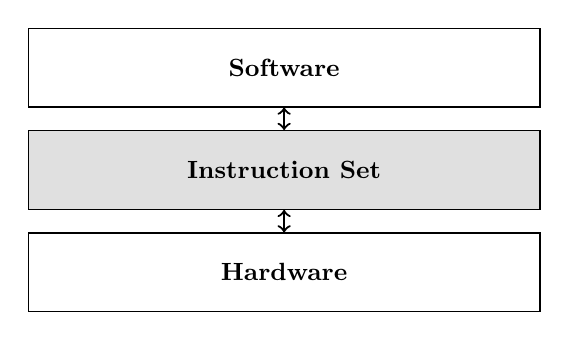
\begin{tikzpicture}[font=\small,
  layer/.style={draw,minimum width=6.5cm,minimum height=1cm,align=center}]
  \node[layer,fill=white] (sw) at (0,2) {\textbf{Software}};
  \node[layer,fill=black!12] (is) at (0,0.7) {\textbf{Instruction Set}};
  \node[layer,fill=white] (hw) at (0,-0.6) {\textbf{Hardware}};
  \draw[<->,thick] (sw) -- (is);
  \draw[<->,thick] (is) -- (hw);
\end{tikzpicture}
\diagramsource{\nolinkurl{02-isa-lecture.pdf}, slide 5 (``The Instruction Set'')}
\end{minipage}
\end{center}
\begin{note}
The instruction set is the \textbf{interface} between software and hardware.
\end{note}

\subsubsection{Instruction execution cycle}

\begin{center}\begin{minipage}{\linewidth}\centering
\begin{tikzpicture}[font=\small,
  block/.style={draw,fill=black!8,minimum width=2.6cm,minimum height=0.9cm,align=center},
  >=Stealth]
  \node[block] (if) at (0,0)    {Instruction\\Fetch};
  \node[block] (id) at (0,-1.3) {Instruction\\Decode};
  \node[block] (of) at (0,-2.6) {Operand\\Fetch};
  \node[block] (ex) at (0,-3.9) {Execute};
  \node[block] (wb) at (0,-5.2) {Write\\Back};
  \draw[->] (if) -- (id);
  \draw[->] (id) -- (of);
  \draw[->] (of) -- (ex);
  \draw[->] (ex) -- (wb);
  \draw[->] (wb.west) -- ++(-1.0,0) |- (if.west);

  \node[right=0.8cm of if] {Obtain the instruction};
  \node[right=0.8cm of id] {Determine action to be performed};
  \node[right=0.8cm of of] {Obtain the operand data};
  \node[right=0.8cm of ex] {Compute the result (update status)};
  \node[right=0.8cm of wb] {Store the result};
\end{tikzpicture}
\diagramsource{\nolinkurl{02-isa-lecture.pdf}, slide 6 (``Instruction execution cycle'')}
\end{minipage}
\end{center}

\subsection{ISA Styles}
\label{sec:isa-styles}

A generic 2-operand operation:
\begin{center}\begin{minipage}{\linewidth}\centering
\begin{tikzpicture}[font=\small,>=Stealth]
  \node[draw,minimum width=3cm,minimum height=1.2cm] (op) at (0,0) {Operation};
  \draw[->] (-0.9,1.3) -- (-0.9,0.65) node[midway,left]{};
  \draw[->] (0.9,1.3) -- (0.9,0.65);
  \node[above] at (-0.9,1.35) {Input1};
  \node[above] at (0.9,1.35) {Input2};
  \draw[->] (0,-0.65) -- (0,-1.3);
  \node[below] at (0,-1.35) {Output};
\end{tikzpicture}
\diagramsource{\nolinkurl{02-isa-lecture.pdf}, slide 7 (``ISA Styles'')}
\end{minipage}
\end{center}

\begin{definition}[ISA style]
ISA styles differ in \emph{where} the operands of an operation live:
\textbf{Stack}, \textbf{Accumulator}, \textbf{Register-Memory} /
\textbf{Memory-Memory}, and \textbf{Register-Register} (a.k.a.\
\emph{load-store}).\HPA[6]{A}{\S A.2, Figures~A.1--A.2}{3}
\end{definition}

\subsubsection{Stack}

\begin{center}\begin{minipage}{\linewidth}\centering
\begin{tikzpicture}[font=\small]
  \draw (-1.3,0.5) rectangle (1.3,1.0) node[midway] {Stack Element};
  \draw (-1.3,0) rectangle (1.3,0.5) node[midway] {Stack Element};
  \node[draw] (tos) at (-2.6,0.75) {TOS};
  \draw[-{Latex}] (tos) -- (-1.3,0.75);
  \pic at (0,-0.6) {valu};
  \draw[-{Latex}] (-0.65,0) -- (-0.65,-0.6);
  \draw[-{Latex}] (1.3,0.75) -- (1.8,0.75) |- (0.65,-0.3) -- (0.65,-0.6);
  \draw[-{Latex}] (0,-1.6) -- (0,-1.95) -| (2.4,1.35) -| (0.65,1.0);
  \node[anchor=west,font=\footnotesize] at (2.7,0.2) {operands: the top two elements};
  \node[anchor=west,font=\footnotesize] at (2.7,-0.3) {result: pushed back on the stack};
\end{tikzpicture}
\diagramsource{\nolinkurl{02-isa-lecture.pdf}, slide 8 (``ISA Styles: Stack''); cf.\ H\&P Fig.~A.1, \hppage{A}{4}}
\end{minipage}
\end{center}
The operands are on top of the stack; the result is pushed back onto the
stack.
\begin{eg}[$C = A + B$]
\leavevmode
\begin{lstlisting}
PUSH A
PUSH B
ADD
POP C     # C = A + B
\end{lstlisting}
\end{eg}
\begin{remark}
\textbf{(+)} Good code density, simple hardware. \quad
\textbf{(--)} Low parallelism, stack is a bottleneck.
\end{remark}

\subsubsection{Accumulator}

\begin{center}\begin{minipage}{\linewidth}\centering
\begin{tikzpicture}[font=\small]
  \draw (-1.1,0.75) rectangle (1.1,1.25) node[midway] {Accumulator};
  \draw (2.4,-0.6) rectangle (4.2,1.4);
  \foreach \y in {-0.1,0.4,0.9} \draw (2.4,\y) -- (4.2,\y);
  \node[fill=white,inner sep=1pt] at (3.3,0.65) {Memory};
  \pic at (0,0) {valu};
  \draw[-{Latex}] (-0.65,0.75) -- (-0.65,0);
  \draw[-{Latex}] (2.4,0.15) -| (0.65,0);
  \draw[-{Latex}] (0,-1) -- (0,-1.3) -| (-1.7,1) -- (-1.1,1);
\end{tikzpicture}
\diagramsource{\nolinkurl{02-isa-lecture.pdf}, slide 9 (``ISA Styles: Accumulator''); cf.\ H\&P Fig.~A.1, \hppage{A}{4}}
\end{minipage}
\end{center}
One accumulator register is used in all operations.
\begin{eg}[$C = A + B$]
\leavevmode
\begin{lstlisting}
LOAD A    ; put A in Accumulator (AC)
ADD B     ; AC <- AC + B
STORE C   ; C <- AC
\end{lstlisting}
\end{eg}
\begin{remark}
\textbf{(+)} Easy to write a compiler, few instructions. \quad
\textbf{(--)} Very high memory traffic, variable CPI.
\end{remark}

\subsubsection{Memory-Memory}

\begin{center}\begin{minipage}{\linewidth}\centering
\begin{tikzpicture}[font=\small]
  \draw (2.2,-1.6) rectangle (4.0,1.0);
  \foreach \y in {-1.1,-0.6,-0.1,0.4} \draw (2.2,\y) -- (4.0,\y);
  \node[fill=white,inner sep=1pt] at (3.1,-0.35) {Memory};
  \pic at (0,0) {valu};
  \draw[-{Latex}] (2.2,0.7) -| (-0.65,0);
  \draw[-{Latex}] (2.2,0.15) -| (0.65,0);
  \draw[-{Latex}] (0,-1) -- (0,-1.35) -- (2.2,-1.35);
\end{tikzpicture}
\diagramsource{\nolinkurl{02-isa-lecture.pdf}, slide 10 (``ISA Styles: Memory-memory'')}
\end{minipage}
\end{center}
All operands are located in memory.
\begin{eg}[$C = A + B$]
\leavevmode
\begin{lstlisting}
ADD C, A, B    ; C <- A + B   (all three in memory)
\end{lstlisting}
\end{eg}
\begin{remark}
\textbf{(+)} Simple to design and understand. \quad
\textbf{(--)} Accumulator-like bottleneck, heavy memory access.
\end{remark}

\subsubsection{Register-Memory}

\begin{center}\begin{minipage}{\linewidth}\centering
\begin{tikzpicture}[font=\small]
  \draw (-1.1,1.2) rectangle (1.1,1.6) node[midway] {Register};
  \draw (-1.1,0.8) rectangle (1.1,1.2) node[midway] {Register};
  \draw (-1.1,0.4) rectangle (1.1,0.8) node[midway] {Register};
  \pic at (0,0) {valu};
  \draw (2.4,-1.0) rectangle (4.2,1.4);
  \foreach \y in {-0.5,0.0,0.5} \draw (2.4,\y) -- (4.2,\y);
  \node[fill=white,inner sep=1pt] at (3.3,0.25) {Memory};
  \draw[-{Latex}] (-0.65,0.4) -- (-0.65,0);
  \draw[-{Latex}] (2.4,0.2) -| (0.65,0);
  \draw[-{Latex}] (0,-1) -- (0,-1.3) -| (-1.7,1.4) -- (-1.1,1.4);
\end{tikzpicture}
\diagramsource{\nolinkurl{02-isa-lecture.pdf}, slide 11 (``ISA Styles: Register-Memory''); cf.\ H\&P Fig.~A.1, \hppage{A}{4}}
\end{minipage}
\end{center}
Inputs/outputs can be either a register or memory.
\begin{eg}[$C = A + B$]
\leavevmode
\begin{lstlisting}
LOAD  R1, A
ADD   R3, R1, B    ; R3 <- R1 + mem[B]
STORE R3, C
\end{lstlisting}
\end{eg}

\subsubsection{Register-Register (Load-Store)}

\begin{center}\begin{minipage}{\linewidth}\centering
\begin{tikzpicture}[font=\small]
  \draw (-1.1,1.2) rectangle (1.1,1.6) node[midway] {Register};
  \draw (-1.1,0.8) rectangle (1.1,1.2) node[midway] {Register};
  \draw (-1.1,0.4) rectangle (1.1,0.8) node[midway] {Register};
  \pic at (0,0) {valu};
  \draw[-{Latex}] (-0.65,0.4) -- (-0.65,0);
  \draw[-{Latex}] (0.65,0.4) -- (0.65,0);
  \draw[-{Latex}] (0,-1) -- (0,-1.3) -| (-1.7,1.4) -- (-1.1,1.4);
\end{tikzpicture}
\diagramsource{\nolinkurl{02-isa-lecture.pdf}, slide 12 (``ISA Styles: Register-Register''); cf.\ H\&P Fig.~A.1, \hppage{A}{4}}
\end{minipage}
\end{center}
All operations are on registers; dedicated \texttt{Load}/\texttt{Store}
instructions access memory.
\begin{eg}[$C = A + B$]
\leavevmode
\begin{lstlisting}
LOAD  R1, A
LOAD  R2, B
ADD   R3, R1, R2
STORE R3, C
\end{lstlisting}
\end{eg}

\subsubsection{Historical examples}

\begin{center}
\begin{tabular}{@{}llll@{}}
\toprule
Machine & \#GPRs & Architecture style & Year \\
\midrule
Motorola 6800 & 2  & Accumulator                    & 1974 \\
DEC VAX       & 16 & Register-Memory / Memory-Memory & 1977 \\
Intel 8086    & 1  & Extended Accumulator            & 1978 \\
Motorola 68000& 16 & Register-Memory                 & 1980 \\
Intel 80386   & 32 & \textcolor{red}{Register-Memory}& 1985 \\
Power PC      & 32 & \textcolor{blue}{Load-Store}    & 1992 \\
Dec Alpha     & 32 & Load-Store                      & 1992 \\
\bottomrule
\end{tabular}
\end{center}

\subsubsection{Other ISA styles}

\begin{itemize}
  \item \textbf{High-level-language architecture} (e.g.\ Burroughs B5000,
  1960s): instructions map closely to HLL constructs. Fell out of favor due
  to a lack of effective compilers to exploit it.
  \item \textbf{Reduced Instruction Set (RISC) architecture}: simplify the
  hardware, the instruction set, and the instruction format; rely on the
  compiler to synthesize complex operations from simple ones. (Covered in
  detail below.)
\end{itemize}

\subsection{Instruction Set Design}
\label{sec:isa-design}

The design of an instruction set is critical to the operation of a computer
system, and includes many aspects:
\begin{itemize}
  \item Operation repertoire
  \item Addressing modes
  \item Data types
  \item Instruction format
  \item Registers
\end{itemize}

\subsubsection{Simple instruction format}

\begin{center}\begin{minipage}{\linewidth}\centering
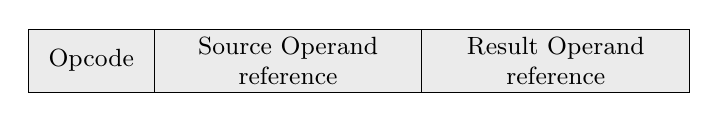
\begin{tikzpicture}[font=\small]
  \draw[fill=black!8] (0,0) rectangle ++(1.6,0.8) node[midway]{Opcode};
  \draw[fill=black!8] (1.6,0) rectangle ++(3.4,0.8) node[midway,align=center]{Source Operand\\reference};
  \draw[fill=black!8] (5,0) rectangle ++(3.4,0.8) node[midway,align=center]{Result Operand\\reference};
\end{tikzpicture}
\diagramsource{\nolinkurl{02-isa-lecture.pdf}, slide 16 (``Simple format'')}
\end{minipage}
\end{center}

\begin{definition}[Instruction fields]
\leavevmode
\begin{itemize}
  \item \textbf{Operation Code}: the operation to be performed by the
  processor.
  \item \textbf{Source Operand Reference}: input(s) of the operation --- one
  or more source operands can be involved.
  \item \textbf{Result Operand Reference}: result of the operation.
\end{itemize}
\end{definition}

\subsubsection{Instruction types}

Can be classified into 4 types:\HPA[16]{A}{\S A.5, Figure~A.13}{14}
\begin{itemize}
  \item \textbf{Data processing}: Arithmetic, Logic \quad (e.g.\ \texttt{ADD},
  \texttt{SUB}, \texttt{AND}, \texttt{OR}, \dots)
  \item \textbf{Data storage}: Move data from/to memory \quad (e.g.\
  \texttt{LD}, \texttt{ST})
  \item \textbf{Data movement}: Register and register/IO \quad (e.g.\
  \texttt{MOV})
  \item \textbf{Control}: Test and branch \quad (e.g.\ \texttt{JMP},
  \texttt{CMP})
\end{itemize}

\begin{explanation}
\emph{``There must certainly be instructions for performing the fundamental
arithmetic operations''} --- Burkes, Goldstine and Von Neumann, 1947.
How many programs have an \texttt{IF} statement? $\to$ branch instructions.
How many have a \texttt{Call} statement? $\to$ call/return instructions. How
many programs access memory? \dots and so on: this is how an ISA's operation
repertoire is decided.
\end{explanation}

\subsubsection{Operator types}

\begin{center}
\begin{tabular}{@{}p{3.2cm}p{10.5cm}@{}}
\toprule
Operator type & Example \\
\midrule
Arithmetic \& Logical & Integer arithmetic and logical operations: add, and,
subtract \dots \\
Data transfer & Loads-stores (move instructions on machines with memory
addressing) \\
Control & Branch, jump, procedure call and return, trap \\
System & Operating system call, virtual memory management instructions \\
Floating point & Floating point instructions: add, multiply \\
Decimal & Decimal add, decimal multiply, decimal-to-character conversion \\
String & String move, string compare, string search \\
Graphic & Pixel operations, compression/decompression operations \\
\bottomrule
\end{tabular}
\end{center}

\begin{remark}
Arithmetic, logical, data transfer and control are almost standard
categories for all machines. System instructions are required for
multi-programming environments (support varies). Others can be primitives
(e.g.\ decimal and string on IBM 360 and VAX), provided by a co-processor,
or synthesized by the compiler.
\end{remark}

\subsection{Addressing Modes}
\label{sec:addressing-modes}

\begin{definition}[Addressing mode]
The way the processor refers to the operands is called the
\textbf{addressing mode}.\HPA[11]{A}{\S A.3, Figure~A.6}{9}
\end{definition}
Addressing modes can be classified based on:
\begin{itemize}
  \item \textbf{The source of data}: immediate, registers, memory.
  \item \textbf{The address calculation}: direct, indirect, indexed.
\end{itemize}

\begin{center}
\begin{tabular}{@{}p{4cm}p{7cm}l@{}}
\toprule
Mode & Description & Example \\
\midrule
Immediate & The operand is put in the instruction. & \texttt{ADD R0,\#10} \\
Register & The index of the register containing the operand is specified in
the instruction. & \texttt{ADD R0,R1} \\
Direct & The address of the operand is put in the instruction. & \texttt{ADD
R0,(100)} \\
Register Indirect & The address of the operand is put \emph{in the register}
specified in the instruction. & \texttt{ADD R0,(R1)} \\
Displacement & The address of the operand is Base register $+$
Displacement. & \texttt{LD R1,100(R2)} \\
Indexed & The address of the operand is Base register $+$ Index register. &
\texttt{ADD R3,(R1+R2)} \\
\bottomrule
\end{tabular}
\end{center}

Generic notation (pseudo-RTL) for the same set of modes:

\begin{center}
\begin{tabular}{@{}ll@{}}
\toprule
Mode & Example \\
\midrule
Immediate       & \texttt{add r1 = r2 + 5} \\
Register        & \texttt{add r1 = r2 + r3} \\
Direct          & \texttt{load r1 = M[4000]} \\
Register Indirect & \texttt{add r1 = r2 + M[r2]} \\
Displacement    & \texttt{load r1 = M[r2 + 4000]} \\
Indexed/Base    & \texttt{add r1 = r3 + M[r2 + r3]} \\
Memory Indirect & \texttt{load r1 = M[M[r2]]} \\
PC Relative     & \texttt{branch r1 < r3, 1000} \\
Scaled          & \texttt{load r1 = M[100 + r3 + r4*d]} \\
\bottomrule
\end{tabular}
\end{center}

\subsubsection{Addressing mode usage (SPEC89 on VAX)}

\begin{center}\begin{minipage}{\linewidth}\centering
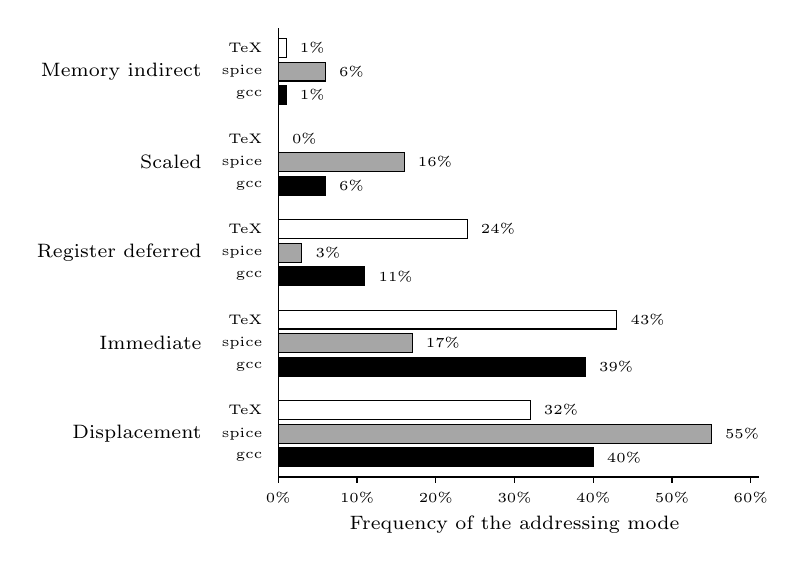
\begin{tikzpicture}[font=\scriptsize]
  \node[anchor=east] at (-0.85,-0.300) {Memory indirect};
  \node[anchor=east,font=\tiny] at (-0.08,0.000) {TeX};
  \draw[fill=white] (0,-0.120) rectangle (0.10,0.120);
  \node[anchor=west,font=\tiny] at (0.15,0.000) {1\%};
  \node[anchor=east,font=\tiny] at (-0.08,-0.300) {spice};
  \draw[fill=black!35] (0,-0.420) rectangle (0.60,-0.180);
  \node[anchor=west,font=\tiny] at (0.65,-0.300) {6\%};
  \node[anchor=east,font=\tiny] at (-0.08,-0.600) {gcc};
  \draw[fill=black] (0,-0.720) rectangle (0.10,-0.480);
  \node[anchor=west,font=\tiny] at (0.15,-0.600) {1\%};
  \node[anchor=east] at (-0.85,-1.450) {Scaled};
  \node[anchor=east,font=\tiny] at (-0.08,-1.150) {TeX};
  \node[anchor=west,font=\tiny] at (0.05,-1.150) {0\%};
  \node[anchor=east,font=\tiny] at (-0.08,-1.450) {spice};
  \draw[fill=black!35] (0,-1.570) rectangle (1.60,-1.330);
  \node[anchor=west,font=\tiny] at (1.65,-1.450) {16\%};
  \node[anchor=east,font=\tiny] at (-0.08,-1.750) {gcc};
  \draw[fill=black] (0,-1.870) rectangle (0.60,-1.630);
  \node[anchor=west,font=\tiny] at (0.65,-1.750) {6\%};
  \node[anchor=east] at (-0.85,-2.600) {Register deferred};
  \node[anchor=east,font=\tiny] at (-0.08,-2.300) {TeX};
  \draw[fill=white] (0,-2.420) rectangle (2.40,-2.180);
  \node[anchor=west,font=\tiny] at (2.45,-2.300) {24\%};
  \node[anchor=east,font=\tiny] at (-0.08,-2.600) {spice};
  \draw[fill=black!35] (0,-2.720) rectangle (0.30,-2.480);
  \node[anchor=west,font=\tiny] at (0.35,-2.600) {3\%};
  \node[anchor=east,font=\tiny] at (-0.08,-2.900) {gcc};
  \draw[fill=black] (0,-3.020) rectangle (1.10,-2.780);
  \node[anchor=west,font=\tiny] at (1.15,-2.900) {11\%};
  \node[anchor=east] at (-0.85,-3.750) {Immediate};
  \node[anchor=east,font=\tiny] at (-0.08,-3.450) {TeX};
  \draw[fill=white] (0,-3.570) rectangle (4.30,-3.330);
  \node[anchor=west,font=\tiny] at (4.35,-3.450) {43\%};
  \node[anchor=east,font=\tiny] at (-0.08,-3.750) {spice};
  \draw[fill=black!35] (0,-3.870) rectangle (1.70,-3.630);
  \node[anchor=west,font=\tiny] at (1.75,-3.750) {17\%};
  \node[anchor=east,font=\tiny] at (-0.08,-4.050) {gcc};
  \draw[fill=black] (0,-4.170) rectangle (3.90,-3.930);
  \node[anchor=west,font=\tiny] at (3.95,-4.050) {39\%};
  \node[anchor=east] at (-0.85,-4.900) {Displacement};
  \node[anchor=east,font=\tiny] at (-0.08,-4.600) {TeX};
  \draw[fill=white] (0,-4.720) rectangle (3.20,-4.480);
  \node[anchor=west,font=\tiny] at (3.25,-4.600) {32\%};
  \node[anchor=east,font=\tiny] at (-0.08,-4.900) {spice};
  \draw[fill=black!35] (0,-5.020) rectangle (5.50,-4.780);
  \node[anchor=west,font=\tiny] at (5.55,-4.900) {55\%};
  \node[anchor=east,font=\tiny] at (-0.08,-5.200) {gcc};
  \draw[fill=black] (0,-5.320) rectangle (4.00,-5.080);
  \node[anchor=west,font=\tiny] at (4.05,-5.200) {40\%};
  \draw (0,0.25) -- (0,-5.45) -- (6.1,-5.45);
  \draw (0.0,-5.45) -- (0.0,-5.52) node[below,font=\tiny] {0\%};
  \draw (1.0,-5.45) -- (1.0,-5.52) node[below,font=\tiny] {10\%};
  \draw (2.0,-5.45) -- (2.0,-5.52) node[below,font=\tiny] {20\%};
  \draw (3.0,-5.45) -- (3.0,-5.52) node[below,font=\tiny] {30\%};
  \draw (4.0,-5.45) -- (4.0,-5.52) node[below,font=\tiny] {40\%};
  \draw (5.0,-5.45) -- (5.0,-5.52) node[below,font=\tiny] {50\%};
  \draw (6.0,-5.45) -- (6.0,-5.52) node[below,font=\tiny] {60\%};
  \node at (3,-6.05) {Frequency of the addressing mode};
\end{tikzpicture}
\diagramsource{\nolinkurl{02-isa-lecture.pdf}, slide 25 (``Addressing mode use''); values checked against H\&P Fig.~A.7, \hppage{A}{11}}
\end{minipage}
\end{center}
\emph{Focus on immediate and displacement modes since they are used the
most} across TeX, spice, and gcc.\HPA[13]{A}{\S A.3, Figures~A.7--A.10}{11}

\subsubsection{Displacement value size}

Measured as number of bits needed; both integer-average and
floating-point-average workloads show most displacement values fit in a
small number of bits, with the bulk of accesses needing $\le 15$ bits and a
long tail:

\begin{center}\begin{minipage}{\linewidth}\centering
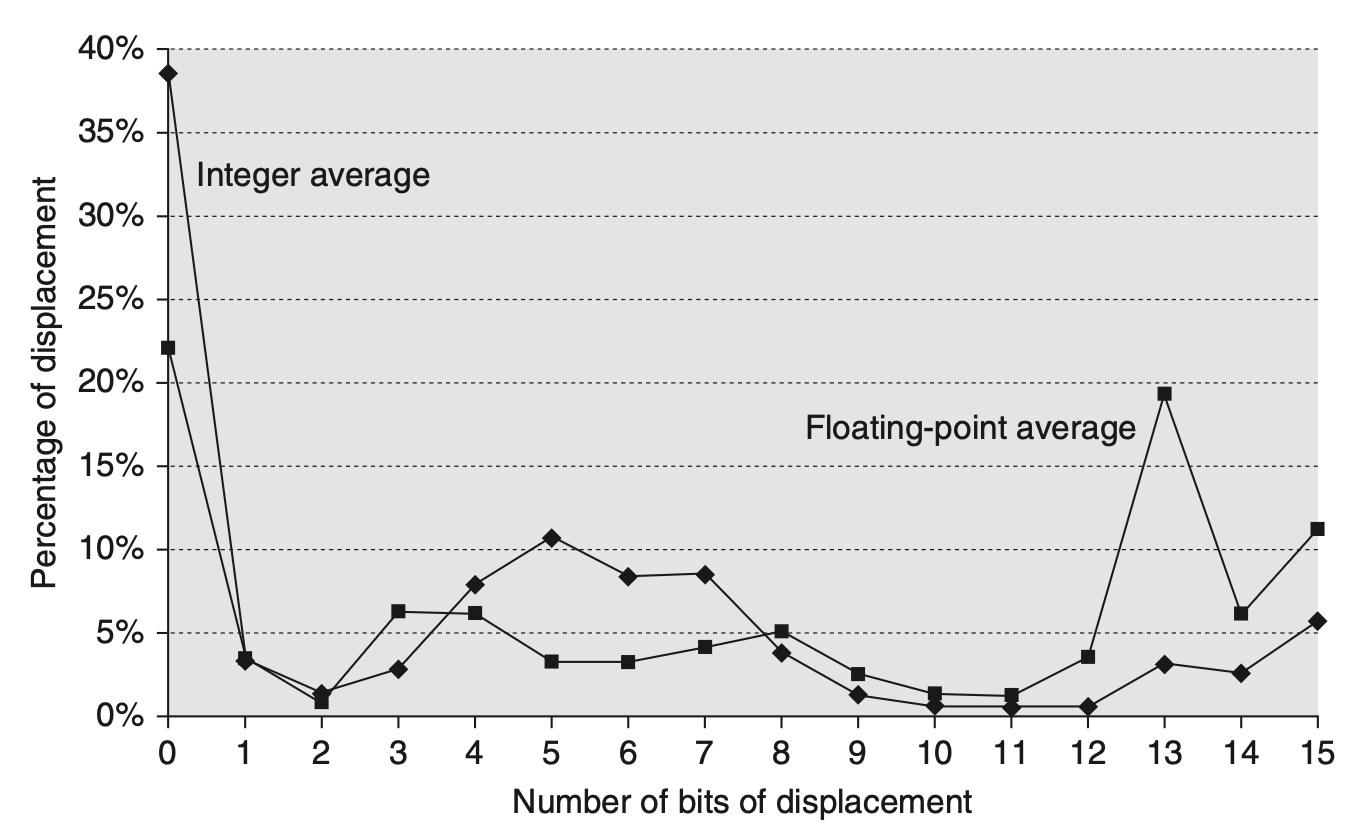
\includegraphics[width=0.8\linewidth]{assets/figures/diag-21.png}
\diagramsource{H\&P Fig.~A.8, \hppage{A}{12} (image supplied by the note-taker); the same chart as \nolinkurl{02-isa-lecture.pdf}, slide 26 (``Addressing mode'')}
\end{minipage}
\end{center}

\subsubsection{Design questions raised by addressing modes}

\begin{itemize}
  \item Is Memory-indirect addressing necessary?
  \item Is Scaled addressing necessary?
  \item Is Register addressing necessary?
  \item How long should a displacement value be?
  \item How long should an immediate value be?
\end{itemize}

\subsection{Operand Types and Sizes}
\label{sec:operands}

\begin{itemize}
  \item \textbf{Character}:
  \begin{itemize}
    \item ASCII (8-bit): almost always used.
    \item Unicode (16-bit): sometimes.
  \end{itemize}
  \item \textbf{Integer}: 2's complement.
  \begin{itemize}
    \item Short: 16 bit.
    \item Long: 32 bit.
  \end{itemize}
  \item \textbf{Floating point}:
  \begin{itemize}
    \item Single precision: 32 bit.
    \item Double precision: 64 bit.
  \end{itemize}
  \item \textbf{Business}: Binary Coded Decimal (BCD) -- accurately
  represents decimal fractions.
  \item \textbf{DSP}: Fixed point, block floating point.
  \item \textbf{Graphic}: RGBA or XYZW, using 8-bit, 16-bit, or single
  precision floating point components.
\end{itemize}

\begin{remark}
Design questions: Should the CPU support all these operand types? Should it
support very big-size operands? Is DSP data used frequently enough to add
dedicated support? Is BCD used in most operations? How about RGBA?
\end{remark}

\subsection{Instruction Format}
\label{sec:instruction-format}

\begin{itemize}
  \item Instructions must be encoded to binary values.\HPA[24]{A}{\S A.7, Figure~A.18}{21}
  \item This affects the size of the compiled program.
  \item Easy to decode $\Rightarrow$ simple to implement.
  \item Should support as many registers and addressing modes as possible.
\end{itemize}

\begin{center}\begin{minipage}{\linewidth}\centering
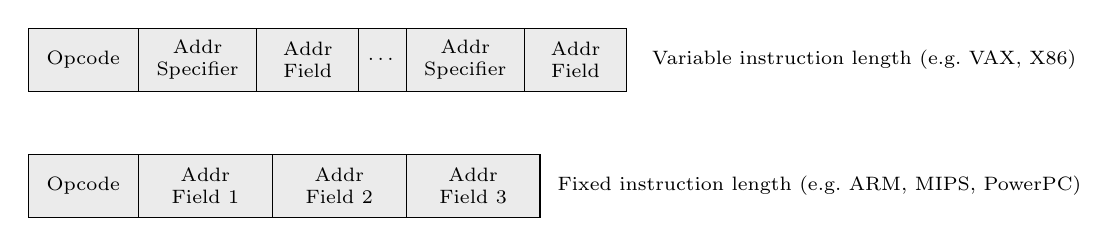
\begin{tikzpicture}[font=\scriptsize]
  % variable length
  \draw[fill=black!8] (0,1.6) rectangle ++(1.4,0.8) node[midway]{Opcode};
  \draw[fill=black!8] (1.4,1.6) rectangle ++(1.5,0.8) node[midway,align=center]{Addr\\Specifier};
  \draw[fill=black!8] (2.9,1.6) rectangle ++(1.3,0.8) node[midway,align=center]{Addr\\Field};
  \draw[fill=black!8] (4.2,1.6) rectangle ++(0.6,0.8) node[midway]{\dots};
  \draw[fill=black!8] (4.8,1.6) rectangle ++(1.5,0.8) node[midway,align=center]{Addr\\Specifier};
  \draw[fill=black!8] (6.3,1.6) rectangle ++(1.3,0.8) node[midway,align=center]{Addr\\Field};
  \node[right] at (7.8,2.0) {Variable instruction length (e.g.\ VAX, X86)};

  % fixed length
  \draw[fill=black!8] (0,0) rectangle ++(1.4,0.8) node[midway]{Opcode};
  \draw[fill=black!8] (1.4,0) rectangle ++(1.7,0.8) node[midway,align=center]{Addr\\Field 1};
  \draw[fill=black!8] (3.1,0) rectangle ++(1.7,0.8) node[midway,align=center]{Addr\\Field 2};
  \draw[fill=black!8] (4.8,0) rectangle ++(1.7,0.8) node[midway,align=center]{Addr\\Field 3};
  \node[right] at (6.6,0.4) {Fixed instruction length (e.g.\ ARM, MIPS, PowerPC)};
\end{tikzpicture}
\diagramsource{\nolinkurl{02-isa-lecture.pdf}, slide 33 (``Instruction format''); cf.\ H\&P Fig.~A.18, \hppage{A}{22}}
\end{minipage}
\end{center}

\begin{note}
\textbf{Hybrid}: to gain high code density while keeping decode simple, use
2 types of fixed-length instructions (e.g.\ MIPS16, Thumb).
\end{note}

\subsubsection{Register file}

\begin{itemize}
  \item Register is the fastest memory element.
  \item Registers cost much more (per bit) than main memory.
  \item Registers are flexible for the compiler to use.
  \item More registers need more bits to encode in each instruction.
  \item A register file with more locations can be slower to access.
  \item Open design question: how many locations in the register file is
  most effective?
\end{itemize}

\subsection{CISC vs.\ RISC}
\label{sec:cisc-risc}

\subsubsection{Complex Instruction Set Computer (CISC)}

\begin{definition}[CISC]
A \emph{Complex Instruction Set Computer} emphasizes doing more with each
instruction, so programs need fewer instructions (more compact code).
\end{definition}
\begin{itemize}
  \item Emphasizes doing more with each instruction $\Rightarrow$ fewer
  instructions per program (more compact code).
  \item Motivated by the \textbf{high cost of memory} and hard-disk capacity
  when original CISC architectures were proposed:
  \begin{itemize}
    \item M6800: 16K RAM = \$500, 40M hard disk = \$55{,}000.
    \item M68000: 64K RAM = \$200, 10M HD = \$5{,}000.
  \end{itemize}
  \item Original CISC architectures evolved with faster, more complex CPU
  designs, but backward instruction-set compatibility had to be maintained.
  \item Wide variety of addressing modes: 14 in MC68000, 25 in MC68020.
  \item A number of instruction modes for the location and number of
  operands: the VAX has 0- through 3-address instructions.
  \item Variable-length instruction encoding.
\end{itemize}

\begin{eg}[Motorola 680X0]
18 addressing modes (data/address
register direct, immediate, absolute short/long, address register indirect
with post-/pre-increment, displacement, indexed, memory indirect
pre-/post-indexed, PC-relative variants, \dots). GPR ISA (Register-Memory).
Operand size ranges from 1 to 32 bits (1, 2, 4, 8, 10, or 16 bytes).
Instructions are stored in 16-bit words; the smallest instruction is 2 bytes
(one word); the longest is 5 words (10 bytes).
\end{eg}

\begin{eg}[Intel IA-32, x86 (80386)]
12 addressing modes
(register, immediate, direct, base, base+displacement,
index+displacement, scaled-index+displacement, based index, based scaled
index, based index+displacement, based scaled index+displacement,
relative). GPR ISA (Register-Memory). Operand sizes 8, 16, 32, 48, 64, or 80
bits; also supports string operations. The smallest instruction is one
byte; the longest is 12 bytes. The first bytes generally contain the
opcode, mode specifiers, and register fields; the remainder are for address
displacement and immediate data.
\end{eg}

\subsubsection{Reduced Instruction Set Computer (RISC)}

\begin{definition}[RISC]
A \emph{Reduced Instruction Set Computer} focuses on reducing the number and
complexity of instructions, aiming for $\CPI \le 1$.\HPA[39]{A}{\S A.9}{32}
\end{definition}
\begin{itemize}
  \item Focuses on reducing the number and complexity of instructions.
  \item Reduced CPI: goal of at least one instruction per clock cycle
  (\textcolor{blue}{CPI $=1$ or less}).
  \item Designed with pipelining in mind.
  \item Fixed-length instruction encoding.
  \item Only load and store instructions access memory.
  \item \textcolor{blue}{(Thus more instructions are executed than CISC.)}
  \item Simplified addressing modes -- usually limited to immediate,
  register indirect, register displacement, indexed.
  \item Delayed loads and branches.
  \item Instruction pre-fetch and speculative execution.
  \item Examples: MIPS, SPARC, PowerPC, Alpha.
\end{itemize}

\begin{eg}[HP Precision Architecture (HP PA-RISC)]
7 addressing
modes: register, immediate, base with displacement, base with scaled index
and displacement, predecrement, postincrement, PC-relative. Five operand
sizes ranging in powers of two from 1 to 16 bytes. Instruction set has 12
different formats, all 32 bits in length.
\end{eg}

\begin{eg}[Alpha AXP]
4 addressing modes: register direct,
immediate, register indirect with displacement, PC-relative. Four operand
sizes: 1, 2, 4, or 8 bytes. Instruction set has 7 different formats, all 32
bits in length.
\end{eg}

\subsection{Case Study: MIPS}
\label{sec:mips}

\subsubsection{Overview}

\begin{itemize}
  \item Instruction categories: Load/Store, Computational, Jump and Branch,
  Floating Point (coprocessor), Memory Management, Special.
  \item 3 instruction formats: all \textbf{32 bits wide}.
\end{itemize}

\begin{center}\begin{minipage}{\linewidth}\centering
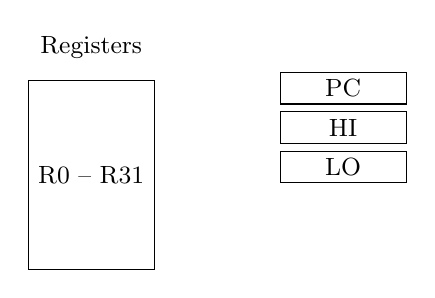
\begin{tikzpicture}[font=\small]
  \node[draw,minimum width=1.6cm,minimum height=2.4cm,align=center] (regs) at (0,0) {R0 -- R31};
  \node[above] at (0,1.35) {Registers};
  \draw[draw,minimum width=1.6cm] (2.4,0.9) rectangle ++(1.6,0.4) node[midway]{PC};
  \draw[draw,minimum width=1.6cm] (2.4,0.4) rectangle ++(1.6,0.4) node[midway]{HI};
  \draw[draw,minimum width=1.6cm] (2.4,-0.1) rectangle ++(1.6,0.4) node[midway]{LO};
\end{tikzpicture}
\diagramsource{\nolinkurl{02-isa-lecture.pdf}, slide 42 (``The MIPS ISA'')}
\end{minipage}
\end{center}

\begin{center}\begin{minipage}{\linewidth}\centering
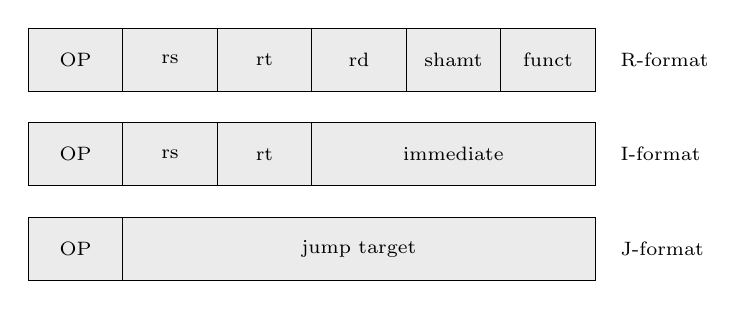
\begin{tikzpicture}[font=\scriptsize]
  \draw[fill=black!8] (0,1.6) rectangle ++(1.2,0.8) node[midway]{OP};
  \draw[fill=black!8] (1.2,1.6) rectangle ++(1.2,0.8) node[midway]{rs};
  \draw[fill=black!8] (2.4,1.6) rectangle ++(1.2,0.8) node[midway]{rt};
  \draw[fill=black!8] (3.6,1.6) rectangle ++(1.2,0.8) node[midway]{rd};
  \draw[fill=black!8] (4.8,1.6) rectangle ++(1.2,0.8) node[midway]{shamt};
  \draw[fill=black!8] (6.0,1.6) rectangle ++(1.2,0.8) node[midway]{funct};
  \node[right] at (7.4,2.0) {R-format};

  \draw[fill=black!8] (0,0.4) rectangle ++(1.2,0.8) node[midway]{OP};
  \draw[fill=black!8] (1.2,0.4) rectangle ++(1.2,0.8) node[midway]{rs};
  \draw[fill=black!8] (2.4,0.4) rectangle ++(1.2,0.8) node[midway]{rt};
  \draw[fill=black!8] (3.6,0.4) rectangle ++(3.6,0.8) node[midway]{immediate};
  \node[right] at (7.4,0.8) {I-format};

  \draw[fill=black!8] (0,-0.8) rectangle ++(1.2,0.8) node[midway]{OP};
  \draw[fill=black!8] (1.2,-0.8) rectangle ++(6,0.8) node[midway]{jump target};
  \node[right] at (7.4,-0.4) {J-format};
\end{tikzpicture}
\diagramsource{\nolinkurl{02-isa-lecture.pdf}, slide 42 (``The MIPS ISA''); cf.\ H\&P Fig.~A.22, \hppage{A}{35}}
\end{minipage}
\end{center}

\subsubsection{MIPS (RISC) design principles}

\begin{noot}{MIPS (RISC) design principles}
\begin{itemize}
  \item \textbf{Simplicity favors regularity}\HPA[39]{A}{\S A.9 (MIPS)}{32}: fixed-size instructions,
  small number of instruction formats, opcode always in the first 6 bits.
  \item \textbf{Smaller is faster}: limited instruction set, limited number
  of registers in the register file, limited number of addressing modes.
  \item \textbf{Make the common case fast}: arithmetic operands from the
  register file (load-store machine), allow instructions to contain
  immediate operands.
  \item \textbf{Good design demands good compromises}: same instruction
  length, single instruction format $\Rightarrow$ compromise of exactly 3
  instruction formats.
\end{itemize}
\end{noot}

\subsubsection{MIPS instruction-class distribution (SPEC2006)}

\begin{center}
\begin{tabular}{@{}lcc@{}}
\toprule
Instruction Class & Integer & Floating Point \\
\midrule
Arithmetic    & 16\% & 48\% \\
Data transfer & 35\% & 36\% \\
Logical       & 12\% & 4\%  \\
Cond.\ Branch & 34\% & 8\%  \\
Jump          & 2\%  & 0\%  \\
\bottomrule
\end{tabular}
\end{center}

\subsubsection{MIPS register convention}

\begin{center}
\begin{tabular}{@{}llll@{}}
\toprule
Name & Register \# & Usage & Preserve on call? \\
\midrule
\$zero      & 0     & constant 0 (hardware)         & n.a. \\
\$at        & 1     & reserved for assembler        & n.a. \\
\$v0--\$v1  & 2--3  & returned values                & no \\
\$a0--\$a3  & 4--7  & arguments                      & yes \\
\$t0--\$t7  & 8--15 & temporaries                    & no \\
\$s0--\$s7  & 16--23& saved values                   & yes \\
\$t8--\$t9  & 24--25& temporaries                    & no \\
\$k0--\$k1  & 26--27& reserved for operating system  & n.a. \\
\$gp        & 28    & global pointer                 & yes \\
\$sp        & 29    & stack pointer                  & yes \\
\$fp        & 30    & frame pointer                  & yes \\
\$ra        & 31    & return address (hardware)      & yes \\
\bottomrule
\end{tabular}
\end{center}

\subsubsection{MIPS endianness}

\begin{center}\begin{minipage}{\linewidth}\centering
\begin{tikzpicture}[font=\scriptsize]
  \draw (1.00,0) rectangle ++(0.7,0.5) node[midway] {\texttt{0A}};
  \draw (1.70,0) rectangle ++(0.7,0.5) node[midway] {\texttt{0B}};
  \draw (2.40,0) rectangle ++(0.7,0.5) node[midway] {\texttt{0C}};
  \draw (3.10,0) rectangle ++(0.7,0.5) node[midway] {\texttt{0D}};
  \node at (2.4,0.75) {Register};
  \draw (-0.80,-1.050) rectangle (0.00,-0.550) node[midway] {\texttt{0A}};
  \node[anchor=east] at (-0.88,-0.800) {$a$};
  \draw[-{Latex[length=2mm]}] (1.35,0) |- (0.00,-0.800);
  \draw (-0.80,-1.600) rectangle (0.00,-1.100) node[midway] {\texttt{0B}};
  \node[anchor=east] at (-0.88,-1.350) {$a+1$};
  \draw[-{Latex[length=2mm]}] (2.05,0) |- (0.00,-1.350);
  \draw (-0.80,-2.150) rectangle (0.00,-1.650) node[midway] {\texttt{0C}};
  \node[anchor=east] at (-0.88,-1.900) {$a+2$};
  \draw[-{Latex[length=2mm]}] (2.75,0) |- (0.00,-1.900);
  \draw (-0.80,-2.700) rectangle (0.00,-2.200) node[midway] {\texttt{0D}};
  \node[anchor=east] at (-0.88,-2.450) {$a+3$};
  \draw[-{Latex[length=2mm]}] (3.45,0) |- (0.00,-2.450);
  \node at (-0.40,-2.95) {Memory};
  \node[font=\small\bfseries] at (2.4,-3.0) {Big-endian};
  \begin{scope}[xshift=7.2cm]
  \draw (1.00,0) rectangle ++(0.7,0.5) node[midway] {\texttt{0A}};
  \draw (1.70,0) rectangle ++(0.7,0.5) node[midway] {\texttt{0B}};
  \draw (2.40,0) rectangle ++(0.7,0.5) node[midway] {\texttt{0C}};
  \draw (3.10,0) rectangle ++(0.7,0.5) node[midway] {\texttt{0D}};
  \node at (2.4,0.75) {Register};
  \draw (4.60,-1.050) rectangle (5.40,-0.550) node[midway] {\texttt{0D}};
  \node[anchor=west] at (5.48,-0.800) {$a$};
  \draw[-{Latex[length=2mm]}] (3.45,0) |- (4.60,-0.800);
  \draw (4.60,-1.600) rectangle (5.40,-1.100) node[midway] {\texttt{0C}};
  \node[anchor=west] at (5.48,-1.350) {$a+1$};
  \draw[-{Latex[length=2mm]}] (2.75,0) |- (4.60,-1.350);
  \draw (4.60,-2.150) rectangle (5.40,-1.650) node[midway] {\texttt{0B}};
  \node[anchor=west] at (5.48,-1.900) {$a+2$};
  \draw[-{Latex[length=2mm]}] (2.05,0) |- (4.60,-1.900);
  \draw (4.60,-2.700) rectangle (5.40,-2.200) node[midway] {\texttt{0A}};
  \node[anchor=west] at (5.48,-2.450) {$a+3$};
  \draw[-{Latex[length=2mm]}] (1.35,0) |- (4.60,-2.450);
  \node at (5.00,-2.95) {Memory};
  \node[font=\small\bfseries] at (2.4,-3.0) {Little-endian};
  \end{scope}
\end{tikzpicture}
\diagramsource{\nolinkurl{02-isa-lecture.pdf}, slide 46 (``MIPS - Endianness''); cf.\ H\&P \S A.3, \hppage{A}{7}}
\end{minipage}
\end{center}

\begin{definition}[Endianness]
\leavevmode
\begin{itemize}
  \item \textbf{Big-endian}: most-significant byte at the lowest address of
  a word.
  \item \textbf{Little-endian}: least-significant byte at the lowest
  address of a word.
  \item \textbf{MIPS is big-endian} in this course. (H\&P's MIPS64 has a mode bit that
  selects big or little endian;\HPA{A}{\S A.9}{34} x86 is little-endian.)
\end{itemize}\HPA{A}{\S A.3}{7}
\end{definition}

\subsubsection{R-Format instructions}

\begin{center}\begin{minipage}{\linewidth}\centering
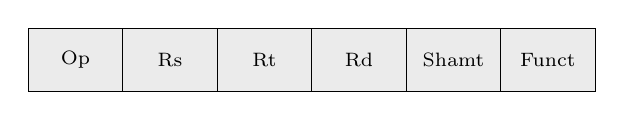
\begin{tikzpicture}[font=\scriptsize]
  \draw[fill=black!8] (0,0) rectangle ++(1.2,0.8) node[midway]{Op};
  \draw[fill=black!8] (1.2,0) rectangle ++(1.2,0.8) node[midway]{Rs};
  \draw[fill=black!8] (2.4,0) rectangle ++(1.2,0.8) node[midway]{Rt};
  \draw[fill=black!8] (3.6,0) rectangle ++(1.2,0.8) node[midway]{Rd};
  \draw[fill=black!8] (4.8,0) rectangle ++(1.2,0.8) node[midway]{Shamt};
  \draw[fill=black!8] (6.0,0) rectangle ++(1.2,0.8) node[midway]{Funct};
\end{tikzpicture}
\diagramsource{\nolinkurl{02-isa-lecture.pdf}, slide 47 (``MIPS R-Format instructions'')}
\end{minipage}
\end{center}

\begin{definition}[R-format fields]
\leavevmode
\begin{itemize}
  \item \textbf{Op}: opcode.
  \item \textbf{Rs}: first source register number.
  \item \textbf{Rt}: second source register number.
  \item \textbf{Rd}: destination register number.
  \item \textbf{Shamt}: shift amount (number of bit positions, left/right).
  \item \textbf{Funct}: extended opcode -- the ALU function that encodes the
  datapath operation. Execution: \texttt{Rd <- Rs func Rt}.
\end{itemize}
\end{definition}

For arithmetic and logical instructions the opcode is always
\texttt{SPECIAL} (\texttt{000000}), and \texttt{Funct} indicates the
specific operation.

\begin{eg}[Encoding \texttt{ADD \$t0, \$s1, \$s2}]
\leavevmode
\begin{lstlisting}
ADD $t0, $s1, $s2
\end{lstlisting}
\begin{center}\begin{minipage}{\linewidth}\centering
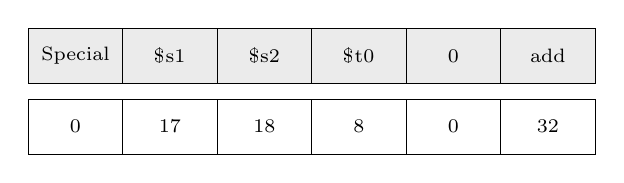
\begin{tikzpicture}[font=\scriptsize]
  \foreach \x/\w/\lab in {0/1.2/Special,1.2/1.2/{\$s1},2.4/1.2/{\$s2},3.6/1.2/{\$t0},4.8/1.2/0,6.0/1.2/add}
    \draw[fill=black!8] (\x,0.9) rectangle ++(\w,0.7) node[midway]{\lab};
  \foreach \x/\w/\lab in {0/1.2/0,1.2/1.2/17,2.4/1.2/18,3.6/1.2/8,4.8/1.2/0,6.0/1.2/32}
    \draw[fill=white] (\x,0) rectangle ++(\w,0.7) node[midway]{\lab};
\end{tikzpicture}
\diagramsource{\nolinkurl{02-isa-lecture.pdf}, slide 49 (``Arithmetic instruction'')}
\end{minipage}
\end{center}
Binary: \texttt{000000 10001 10010 01000 00000 100000} \quad =\quad
\texttt{0x02324020}.
\end{eg}

\subsubsection{Logical operations}

\texttt{AND, OR, XOR, NOR} (bit-wise).
\begin{lstlisting}
OR $t0, $t1, $t2    # $t0 = $t1 | $t2
\end{lstlisting}
Shift left / shift right: \texttt{Shamt} indicates the number of bits to
shift.
\begin{eg}[Shift left logical]
\leavevmode
\begin{lstlisting}
SLL $t2, $s0, 8
\end{lstlisting}
Encoding: \texttt{000000 00000 10000 01010 01000 000000}.
\end{eg}

\texttt{Shift Right Arithmetic (SRA)} uses the MSB as the shift-in bit
(sign-extending):
\begin{eg}[Shift right arithmetic]
\leavevmode
\begin{lstlisting}
SRA $t2, $s0, 8
\end{lstlisting}
Encoding: \texttt{000000 00000 10000 01010 01000 000011}.
\end{eg}

\begin{remark}
Design questions: why is there no \texttt{SLA} (shift-left-arithmetic)?
Why is there no \texttt{NOT}?
\end{remark}

\subsubsection{Jump register}

Uses \textbf{register indirect addressing}.
\begin{itemize}
  \item \texttt{JR rs}: jump register. \texttt{Rs} = target address;
  \texttt{Rd}, \texttt{Rt} $= 0$; \texttt{shamt} is a hint field (see the MIPS instruction set reference).
  \item \texttt{JALR rs} / \texttt{JALR rd, rs}: jump and link register.
  \texttt{Rs} = target address; \texttt{Rd} = return address; \texttt{Rt}
  $=0$; \texttt{shamt} is a hint field.
\end{itemize}

\subsubsection{I-Format instructions}

\begin{center}\begin{minipage}{\linewidth}\centering
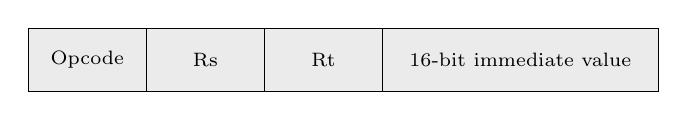
\begin{tikzpicture}[font=\scriptsize]
  \draw[fill=black!8] (0,0) rectangle ++(1.5,0.8) node[midway]{Opcode};
  \draw[fill=black!8] (1.5,0) rectangle ++(1.5,0.8) node[midway]{Rs};
  \draw[fill=black!8] (3.0,0) rectangle ++(1.5,0.8) node[midway]{Rt};
  \draw[fill=black!8] (4.5,0) rectangle ++(3.5,0.8) node[midway]{16-bit immediate value};
\end{tikzpicture}
\diagramsource{\nolinkurl{02-isa-lecture.pdf}, slide 53 (``MIPS I-Format instructions'')}
\end{minipage}
\end{center}

This format is used for:
\begin{itemize}
  \item Operation with immediate addressing.
  \item Operation with displacement addressing.
  \item Operation with PC-relative addressing.
\end{itemize}

\begin{eg}[Immediate arithmetic and logical]
\texttt{Op}: opcode;
\texttt{Rs}: source register; \texttt{Rt}: destination register;
\texttt{Constant}: immediate value ($-32768$ to $32767$).
\begin{lstlisting}
ADDI $t0, $t1, 0x0005
ORI  $t0, $t1, 0xFF00
\end{lstlisting}
Encodings:
\begin{center}
\texttt{001000 01001 01000 0000000000000101}\\
\texttt{001101 01001 01000 1111111100000000}
\end{center}
(Design question: why is there no \texttt{SUBI}?)
\end{eg}

\begin{eg}[Load-Store (displacement)]
\texttt{Rs}: base register number;
16-bit immediate value: offset added to the base address in \texttt{Rs}.
Effective address $EA = Rs + \text{16-bit immediate value}$. For loads,
\texttt{Rt} is the destination register; for stores, \texttt{Rt} is the
value stored to the \texttt{EA} in memory.
\begin{lstlisting}
LW $t0, 16($t1)
SW $t0, 16($t1)
\end{lstlisting}
Encodings:
\begin{center}
\texttt{100011 01001 01000 0000000000010000}\\
\texttt{101011 01001 01000 0000000000010000}
\end{center}
\end{eg}

\begin{eg}[PC-relative (near branches)]
\texttt{Rs}, \texttt{Rt}: source
register numbers; target address $=$ \texttt{PC} $+$ offset $\times 4$ (PC
already incremented by 4 at this time).
\begin{lstlisting}
BEQ $s0, $s1, 256    # if ($s0 == $s1) goto PC + 256*4;
\end{lstlisting}
Encoding: \texttt{000100 10000 10001 0000000100000000}.
\end{eg}

\subsubsection{J-Format instructions}

\begin{center}\begin{minipage}{\linewidth}\centering
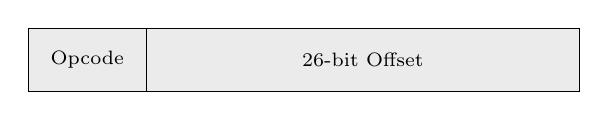
\begin{tikzpicture}[font=\scriptsize]
  \draw[fill=black!8] (0,0) rectangle ++(1.5,0.8) node[midway]{Opcode};
  \draw[fill=black!8] (1.5,0) rectangle ++(5.5,0.8) node[midway]{26-bit Offset};
\end{tikzpicture}
\diagramsource{\nolinkurl{02-isa-lecture.pdf}, slide 59 (``MIPS J-format Instructions'')}
\end{minipage}
\end{center}

Used for \texttt{J} and \texttt{JAL} -- \textbf{pseudo-direct addressing}.
Cannot fit a 32-bit value in the instruction, so target address $=
PC_{31\ldots28} \,\Vert\, (\text{26-bit offset} \times 4)$.
\begin{eg}[Jump]
\leavevmode
\begin{lstlisting}
J 0x01000000
\end{lstlisting}
Encoding: \texttt{000010 01000000000000000000000000}.
\end{eg}

\subsubsection{Moving data without a MOV instruction}

\begin{eg}[Move without MOV]
How to move data from \texttt{\$t0} to \texttt{\$t1} using one MIPS
instruction? MIPS has no dedicated \texttt{MOV}, so it is synthesized:
\[
  \texttt{MOV \$t1, \$t0} \;\equiv\; \texttt{add \$t1, \$t0, \$zero}
\]
\end{eg}

\subsubsection{Atomic operations}

\begin{definition}[Load linked / store conditional]
An atomic Read-Modify-Write operation is built from a pair of instructions:
\texttt{LL} (Load Linked Word) and \texttt{SC} (Store Conditional Word).
\begin{lstlisting}
LL $Rt, offset($Rs)
SC $Rt, offset($Rs)
\end{lstlisting}
If the memory word addressed by \texttt{LL} is modified before the matching
\texttt{SC} to the same address, \texttt{SC} \emph{fails} and returns 0 in
\texttt{\$Rt}. Otherwise, \texttt{SC} stores \texttt{\$Rt} to memory and
returns 1 in \texttt{\$Rt}.\HP{\S5.5}{388}
\end{definition}

\begin{eg}[Atomic swap]
\leavevmode
\begin{lstlisting}
try:  ADD $t0, $zero, $s4   # $t0 = $s4
      LL  $t1, 0($s1)       # $t1 = mem($s1)
      SC  $t0, 0($s1)       # mem($s1) = $t0 (if uncontended)
      BEQ $t0, $zero, try   # if mem($s1) changed meanwhile, retry
                             # else mem($s1) = old $t0
      ADD $s4, $zero, $t1   # $s4 = $t1
\end{lstlisting}
\end{eg}

\subsubsection{Constant (immediate) values}

Small constants are used quite frequently ($\approx 50\%$ of operands in
many common programs):
\begin{eg}[Small and large constants]
\leavevmode
\begin{lstlisting}
# $t0 = 0x1234
ADDI $t0, $zero, 0x1234
\end{lstlisting}
For a 32-bit constant that does not fit in the 16-bit immediate field, use
\texttt{LUI} (Load Upper Immediate) followed by \texttt{ORI}:
\begin{lstlisting}
# $t0 = 0x12345678
LUI $t0, 0x1234
ORI $t0, $t0, 0x5678
\end{lstlisting}
\end{eg}

\subsubsection{Procedure call convention}

\begin{definition}[Procedure call convention]
\leavevmode
\begin{enumerate}
  \item Save the return address.
  \item Save necessary registers.
  \item Callee executes the function.
  \item Restore previously saved registers.
  \item Restore the return address.
  \item Jump to the return address.
\end{enumerate}
\end{definition}
\begin{itemize}
  \item \texttt{JAL label}: jump to a label (procedure); the return address
  is stored in \texttt{\$ra} (register 31).
  \item \texttt{JR}: jump to the address stored in a register.
\end{itemize}

\begin{eg}[Array element swap]
\leavevmode
\begin{lstlisting}
swap(int v[], int k)
{
    int temp;
    temp   = v[k];
    v[k]   = v[k+1];
    v[k+1] = temp;
}
\end{lstlisting}
Assume \texttt{swap} is called as a procedure; \texttt{temp} is register
\texttt{\$15}; arguments in \texttt{\$a1}, \texttt{\$a2}; \texttt{\$16} is a
scratch register.

\begin{lstlisting}
swap:
    addi $sp,$sp,-4     ; create space on stack
    sw   $16, 0($sp)    ; callee-saved register put onto stack
    sll  $t2, $a2,2     ; multiply k by 4
    addu $t2, $a1,$t2   ; address of v[k]
    lw   $15, 0($t2)    ; load v[k]
    lw   $16, 4($t2)    ; load v[k+1]
    sw   $16, 0($t2)    ; store v[k+1] into v[k]
    sw   $15, 4($t2)    ; store old value of v[k] into v[k+1]
    lw   $16, 0($sp)    ; callee-saved register restored from stack
    addi $sp,$sp, 4     ; restore top of stack
    jr   $31            ; return to place that called swap
\end{lstlisting}
\end{eg}

\begin{eg}[Recursive factorial]
\leavevmode
\begin{lstlisting}
fact:
    addi $sp, $sp, -8   # adjust stack for 2 items
    sw   $ra, 4($sp)    # save return address
    sw   $a0, 0($sp)    # save argument

    slti $t0, $a0, 1    # test for n < 1
    beq  $t0, $zero, L1

    addi $v0, $zero, 1  # if so, result is 1
    addi $sp, $sp, 8     #   pop 2 items from stack
    jr   $ra             #   and return

L1: addi $a0, $a0, -1   # else decrement n
    jal  fact             # recursive call

    lw   $a0, 0($sp)    # restore original n
    lw   $ra, 4($sp)    #   and return address
    addi $sp, $sp, 8    # pop 2 items from stack

    mul  $v0, $a0, $v0  # multiply to get result n*fact(n-1)
    jr   $ra             # and return
\end{lstlisting}
\end{eg}

\subsubsection{Reference tables}

\begin{center}
\begin{tabular}{@{}p{2.6cm}p{2.6cm}p{3.3cm}p{4.6cm}@{}}
\toprule
Instruction & Example & Meaning & Comment \\
\midrule
add            & \texttt{add \$1,\$2,\$3}   & \$1 = \$2 + \$3 & 3 operands; exception possible \\
subtract       & \texttt{sub \$1,\$2,\$3}   & \$1 = \$2 -- \$3 & 3 operands; exception possible \\
add immediate  & \texttt{addi \$1,\$2,100}  & \$1 = \$2 + 100 & + constant; exception possible \\
add unsigned   & \texttt{addu \$1,\$2,\$3}  & \$1 = \$2 + \$3 & 3 operands; no exceptions \\
subtract unsigned & \texttt{subu \$1,\$2,\$3} & \$1 = \$2 -- \$3 & 3 operands; no exceptions \\
add imm.\ unsign. & \texttt{addiu \$1,\$2,100} & \$1 = \$2 + 100 & + constant; no exceptions \\
multiply       & \texttt{mult \$2,\$3}      & Hi,Lo = \$2 $\times$ \$3 & 64-bit signed product \\
multiply unsigned & \texttt{multu \$2,\$3}  & Hi,Lo = \$2 $\times$ \$3 & 64-bit unsigned product \\
divide         & \texttt{div \$2,\$3}       & Lo=\$2$\div$\$3, Hi=\$2 mod \$3 & Lo=quotient, Hi=remainder \\
divide unsigned & \texttt{divu \$2,\$3}     & Lo=\$2$\div$\$3, Hi=\$2 mod \$3 & unsigned quotient \& remainder \\
move from Hi   & \texttt{mfhi \$1}          & \$1 = Hi & used to get copy of Hi \\
move from Lo   & \texttt{mflo \$1}          & \$1 = Lo & used to get copy of Lo \\
\bottomrule
\end{tabular}
\end{center}

\begin{center}
\begin{tabular}{@{}p{2.9cm}p{2.5cm}p{3cm}p{4.3cm}@{}}
\toprule
Instruction & Example & Meaning & Comment \\
\midrule
and            & \texttt{and \$1,\$2,\$3}  & \$1=\$2\&\$3       & 3 reg.\ operands; logical AND \\
or             & \texttt{or \$1,\$2,\$3}   & \$1=\$2\textbar\$3 & 3 reg.\ operands; logical OR \\
xor            & \texttt{xor \$1,\$2,\$3}  & \$1=\$2$\oplus$\$3 & 3 reg.\ operands; logical XOR \\
nor            & \texttt{nor \$1,\$2,\$3}  & \$1=$\sim$(\$2\textbar\$3) & 3 reg.\ operands; logical NOR \\
and immediate  & \texttt{andi \$1,\$2,10}  & \$1=\$2\&10        & logical AND reg, constant \\
or immediate   & \texttt{ori \$1,\$2,10}   & \$1=\$2\textbar10  & logical OR reg, constant \\
xor immediate  & \texttt{xori \$1,\$2,10}  & \$1=$\sim$\$2\&$\sim$10 & logical XOR reg, constant \\
shift left logical & \texttt{sll \$1,\$2,10} & \$1=\$2\textless\textless10 & shift left by constant \\
shift right logical & \texttt{srl \$1,\$2,10} & \$1=\$2\textgreater\textgreater10 & shift right by constant \\
shift right arithm. & \texttt{sra \$1,\$2,10} & \$1=\$2\textgreater\textgreater10 & shift right (sign extend) \\
shift left logical (var) & \texttt{sllv \$1,\$2,\$3} & \$1=\$2\textless\textless\$3 & shift left by variable \\
shift right logical (var) & \texttt{srlv \$1,\$2,\$3} & \$1=\$2\textgreater\textgreater\$3 & shift right by variable \\
shift right arithm.\ (var) & \texttt{srav \$1,\$2,\$3} & \$1=\$2\textgreater\textgreater\$3 & shift right arith.\ by variable \\
\bottomrule
\end{tabular}
\end{center}

\begin{center}
\begin{tabular}{@{}ll@{}}
\toprule
Instruction & Comment \\
\midrule
\texttt{SW 500(R4), R3} & Store word \\
\texttt{SH 502(R2), R3} & Store half \\
\texttt{SB 41(R3), R2}  & Store byte \\
\texttt{LW R1, 30(R2)}  & Load word \\
\texttt{LH R1, 40(R3)}  & Load halfword \\
\texttt{LHU R1, 40(R3)} & Load halfword unsigned \\
\texttt{LB R1, 40(R3)}  & Load byte \\
\texttt{LBU R1, 40(R3)} & Load byte unsigned \\
\texttt{LUI R1, 40}     & Load upper immediate (16 bits shifted left by 16) \\
\bottomrule
\end{tabular}
\end{center}

\begin{center}
\begin{tabular}{@{}lll@{}}
\toprule
& & \\
\midrule
Compare and Branch & \texttt{BEQ rs,rt,offset} & if R[rs]==R[rt] then PC-relative branch \\
                    & \texttt{BNE rs,rt,offset} & \dots not-equal ($\neq$) \\
                    & \texttt{BLEZ rs,offset}   & if R[rs] $\le$ 0 then PC-relative branch \\
                    & \texttt{BGTZ rs,offset}   & \dots greater-than ($>$) \\
                    & \texttt{BLTZ rs,offset}   & \dots less-than ($<$) \\
                    & \texttt{BGEZ rs,offset}   & \dots greater-or-equal ($\ge$) \\
\bottomrule
\end{tabular}
\end{center}

\begin{center}
\begin{tabular}{@{}p{2.7cm}p{3cm}p{7.2cm}@{}}
\toprule
Instruction & Example & Meaning \\
\midrule
branch on equal & \texttt{beq \$1,\$2,100} & if (\$1==\$2) go to PC+4+100; equal test; PC-relative branch \\
branch on not eq.\ & \texttt{bne \$1,\$2,100} & if (\$1!=\$2) go to PC+4+100; not-equal test; PC-relative \\
set on less than & \texttt{slt \$1,\$2,\$3} & if (\$2<\$3) \$1=1; else \$1=0; compare less than; 2's comp. \\
set less than imm. & \texttt{slti \$1,\$2,100} & if (\$2<100) \$1=1; else \$1=0; compare~<~constant; 2's comp. \\
set less than uns. & \texttt{sltu \$1,\$2,\$3} & if (\$2<\$3) \$1=1; else \$1=0; compare less than; natural no.\ \\
set l.t.\ imm.\ uns. & \texttt{sltiu \$1,\$2,100} & if (\$2<100) \$1=1; else \$1=0; compare~<~constant; natural \\
jump            & \texttt{j 10000}   & go to 10000; jump to target address \\
jump register   & \texttt{jr \$31}   & go to \$31; for switch, procedure return \\
jump and link   & \texttt{jal 10000} & \$31 = PC+4; go to 10000; for procedure call \\
\bottomrule
\end{tabular}
\end{center}

\subsubsection{Assembler directives and example programs}

\begin{definition}[Assembler directives]
Common assembler (GAS/SPIM-style) directives: \texttt{.text} (code
section), \texttt{.data} (data section), \texttt{.globl} (export a label),
\texttt{.word} (a 32-bit word constant), \texttt{.space} (reserve $n$
bytes).
\end{definition}

\begin{eg}[Adding two constants]
\leavevmode
\begin{lstlisting}
.text
.globl main
main:
    li   $t0, 0x2         # $t0 <- 0x2
    li   $t1, 0x3         # $t1 <- 0x3
    addu $t2, $t0, $t1    # $t2 <- ADD($t0, $t1)
\end{lstlisting}
which is equivalent to (\texttt{li} pseudo-instruction expanded):
\begin{lstlisting}
.text
.globl main
main:
    ori  $t0, $0, 0x2     # $t0 <- OR(0, 0x2)
    ori  $t1, $0, 0x3     # $t1 <- OR(0, 0x3)
    addu $t2, $t0, $t1    # $t2 <- ADD($t0, $t1)
\end{lstlisting}
\end{eg}

\begin{eg}[Using labeled data]
\leavevmode
\begin{lstlisting}
.data
n:  .word 0x2
m:  .word 0x3
r:  .space 4

.text
.globl main
main:
    lw   $t0, n            # load n to $t0
    lw   $t1, m            # load m to $t1
    addu $t2, $t0, $t1     # $t2 <- ADD($t0, $t1)
    sw   $t2, r            # store $t2 to r
\end{lstlisting}
\end{eg}

\begin{eg}[Indexing into an array (\texttt{la} + displacement)]
\leavevmode
\begin{lstlisting}
.data
n:  .word 0x2, 0x3, 0x4

.text
.globl main
main:
    la   $t5, n             # load address of n to $t5
    lw   $t0, 0($t5)        # load n[0] to $t0
    lw   $t1, 4($t5)        # load n[1] to $t1
    addu $t2, $t0, $t1      # $t2 <- ADD($t0, $t1)
    sw   $t2, 8($t5)        # store $t2 to n[2]
\end{lstlisting}
\end{eg}

\subsubsection{Using the SPIM simulator}

A typical SPIM (QtSpim) workflow to assemble, run, and debug MIPS code:
\begin{enumerate}
  \item \textbf{Start SPIM}: the window shows the integer/FP register file,
  the program's text segment (disassembly), and a message log.
  \item \textbf{Load a program}: \emph{File $\to$ Reinitialize and Load
  File}, then select your assembly (\texttt{.s}) file.
  \item \textbf{Execute}: step or run; the current instruction is
  highlighted, and register changes from the previous instruction are shown.
  \item \textbf{Inspect data}: the \emph{Data} tab shows the user data
  segment and stack contents in memory.
  \item \textbf{Set a breakpoint}: right-click an instruction in the text
  segment and choose \emph{Set Breakpoint} (e.g.\ at a conditional branch).
  \item \textbf{Single-step}: use the step button (F10) to execute the
  program line by line and watch register/memory state evolve.
\end{enumerate}

\subsubsection{Reference}
\emph{MIPS instruction set reference}, course handout
(\texttt{references/mips-reference-data.pdf}); see also the reformatted
version, \texttt{references/mips-reference-readable.pdf}.

% =============================================================================
\subsection{Textbook Exercises}
\label{sec:isa-tbx}

\begin{tbexercise}[A]{A.7}{48}{\S A.2 and \S A.9, \hppages{A}{3}{6}, \hppages{A}{32}{39}}
For \texttt{for (i = 0; i <= 100; i++) \{ A[i] = B[i] + C; \}}, with \texttt{A},
\texttt{B} arrays of 64-bit integers and \texttt{C}, \texttt{i} 64-bit integers, all
kept in memory (at 1000, 3000, 5000, 7000) except while operated on, and registers
lost between iterations: (a) write the MIPS code; how many instructions are executed,
how many data memory references, what is the code size? (b) The same for x86.
\end{tbexercise}

\begin{tbexercise}[A]{A.8}{48}{\S A.2 and \S A.7, \hppages{A}{21}{24}}
Instructions are 12 bits long with 5-bit register (address) fields (32 registers).
(a) Can you encode 3 two-address, 30 one-address and 45 zero-address instructions?
(b) 3 two-address, 31 one-address and 35 zero-address? Explain. (c) With 3 two-address
and 24 zero-address instructions, what is the maximum number of one-address
instructions?
\end{tbexercise}

\begin{tbexercise}[A]{A.9}{49}{\S A.2, Figure~A.2, \hppages{A}{3}{6}}
$A$--$F$ are in memory; opcodes are 8 bits, memory addresses 64 bits, register
addresses 6 bits. (a) For each ISA style (stack, accumulator, register-memory,
load-store), how many addresses appear in each instruction of $C=A+B$, and what is the
code size? (b) For each style write $C=A+B$; $D=A-E$; $F=C+D$, marking destroyed
operands and overhead instructions; give the code size, bytes moved to and from
memory, and the overhead instructions and bytes.
\end{tbexercise}

\begin{tbexercise}[A]{A.10}{49}{\S A.2, \S A.7, \S A.9}
MIPS has 32 general-purpose and 32 floating-point registers. If registers are good,
are more registers better? List and discuss the trade-offs of increasing their number.
\end{tbexercise}

\begin{tbexercise}[A]{A.11}{50}{\S A.3 (alignment), \hppages{A}{7}{8}}
\texttt{struct foo \{ char a; bool b; int c; double d; short e; float f; double g;
char *cptr; float *fptr; int x; \};} What is its size on a 32-bit machine? What is
the minimum size if the members may be reordered? And on a 64-bit machine?
\end{tbexercise}

\begin{tbexercise}[A]{A.22}{54}{\S A.3 (byte order, alignment), \hppages{A}{7}{8}}
The value \texttt{434F 4D50 5554 4552} (hex) is stored in an aligned 64-bit
doubleword. (a) Write the bytes in big-endian order and the ASCII character of each.
(b) The same in little-endian order. (c) Give all misaligned 2-byte words readable in
big-endian order. (d) Give all misaligned 4-byte words readable in little-endian order.
\end{tbexercise}

